\documentclass{article}

% Language setting
% Replace `english' with e.g. `spanish' to change the document language
\usepackage[french]{babel}
\usepackage[fleqn]{amsmath} % Aligner les équations à gauche


% Set page size and margins
% Replace `letterpaper' with`a4paper' for UK/EU standard size
\usepackage[letterpaper,top=2cm,bottom=2cm,left=3cm,right=3cm,marginparwidth=1.75cm]{geometry}

% Useful packages

\usepackage{amsmath}
\usepackage{graphicx}
\usepackage{subcaption}
\usepackage[colorlinks=true, allcolors=blue]{hyperref}

\title{TD Michelson }
\author{IPESUP - PC }
\date{DATE}

\begin{document}
\maketitle

\section{Rappels de cours}
Michelson (prix Nobel de physique 1907) créa l'interféromètre de Michelson pour tenter de mesurer la vitesse d'entraînement de la lumière dans le référentiel terrestre. 
Cet instrument est de nos jours encore utilisé: la première détection d'ondes gravitationnelles (le 14 septembre 2015) fut réalisée grâce à LIGO, un interféromètre de Michelson géant de plusieurs kilomètres ! \\
Il existe deux réglages du Michelson, en \textbf{lame d'air} et en \textbf{coin d'air}.\\ 
En lame d'air: \\
\begin{itemize}
  \item Les miroirs sont perpendiculaires
  \item Les franges sont localisées à l'infini (penser à regarder "au loin" pour les observer à l'oeil nu)
  \item $\delta = 2ne cos(i)$ 
  \item La figure d'interférences est faite d'anneaux (franges d'égale inclinaison). \\

\end{itemize}

En coin d'air: \\
\begin{itemize}
  \item Les miroirs ne sont pas perpendiculaires (angle $\alpha$). 
  \item Les franges sont situées au voisinage des miroirs. 
  \item $\delta = 2 \alpha x $
  \item Les franges sont des droites parallèles d'égale épaisseur. \\
\end{itemize}

Pour arriver au contact optique ($e=0$), on se place en configuration lame d'air et on rapproche les miroirs de façon à ce que les anneaux convergent vers le centre jusqu'à l'obtention de la teinte plate. 


\begin{figure}[htbp]
  \centering{
  \begin{subfigure}[b]{0.45\textwidth}
      \centering
      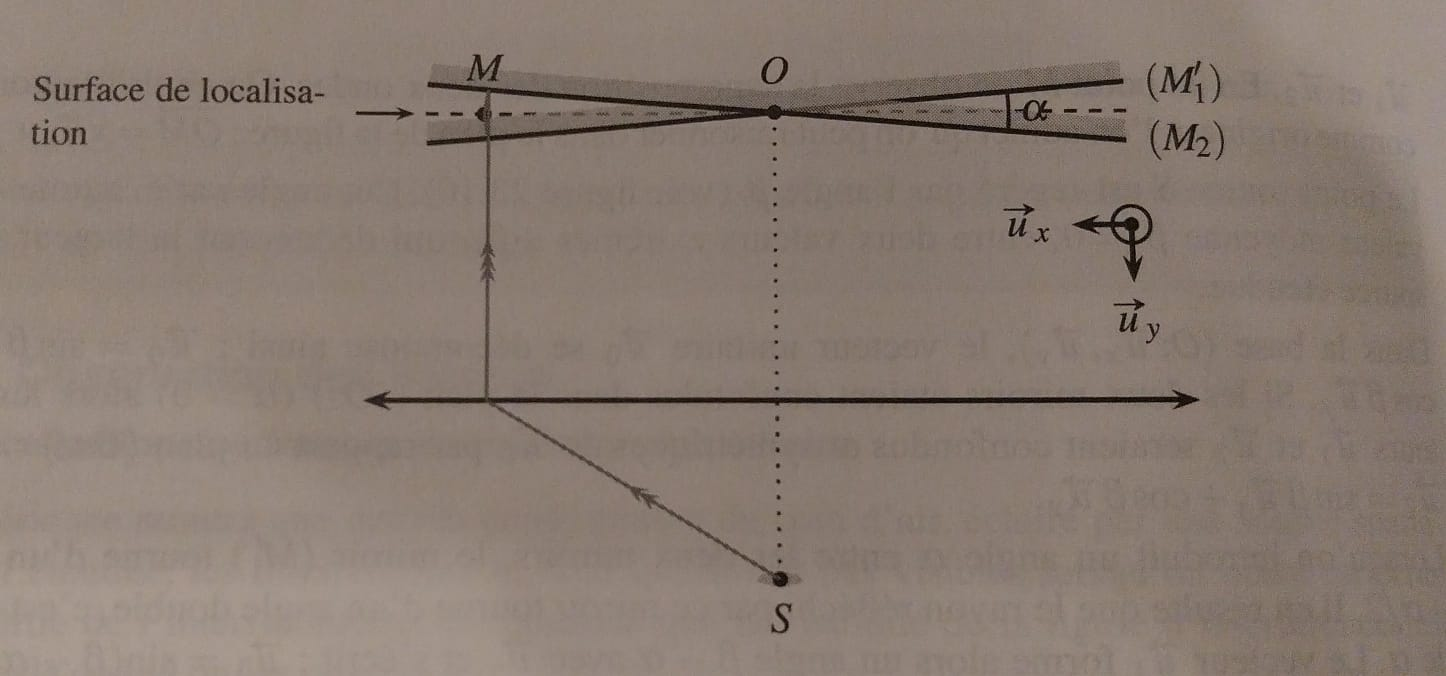
\includegraphics[width=\textwidth]{schema_michelson_coin_d_air.jpg}
      \caption{Michelson réglé en coin d'air}                                              
  \end{subfigure}
  \begin{subfigure}[b]{0.3\textwidth}
      \centering
      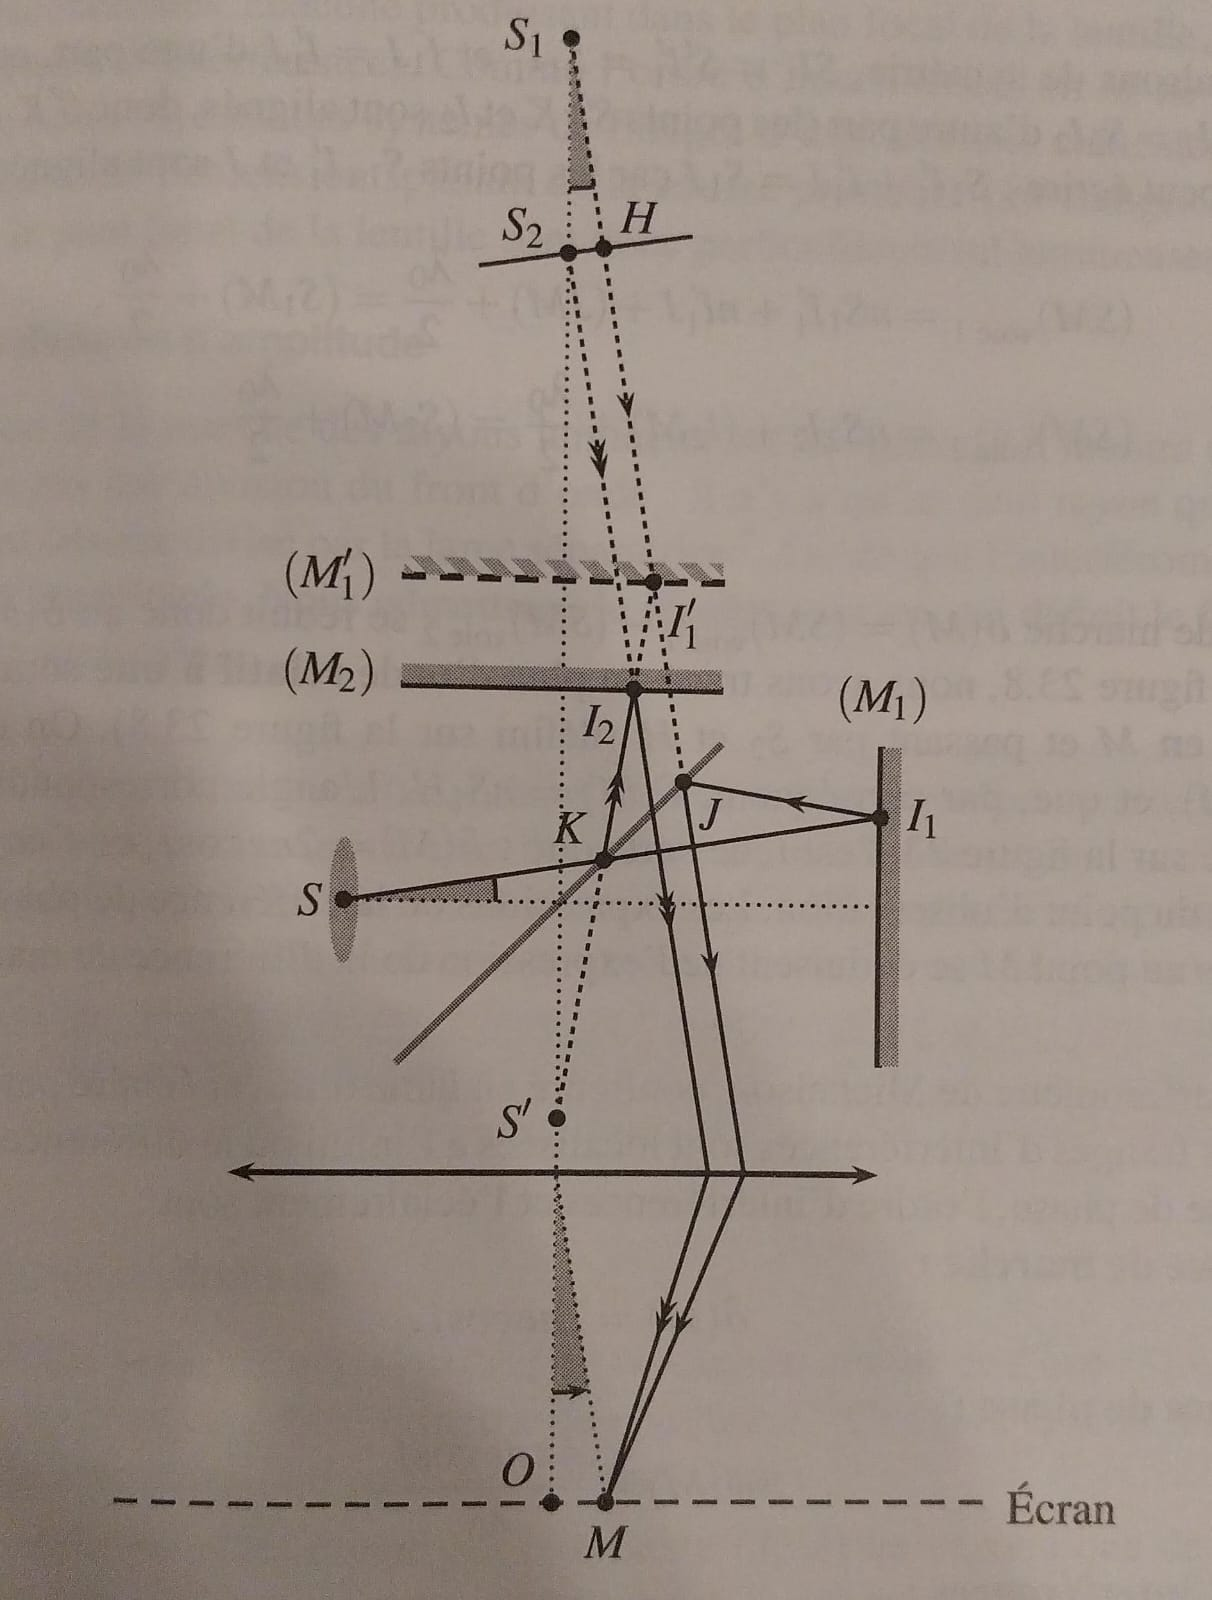
\includegraphics[width=\textwidth]{schema_michelson_lame_d_air.jpg}
      \caption{Michelson réglé en lame d'air } 
  \end{subfigure}}
  \caption{Deux manières de régler un Michelson}
\end{figure}




\begin{figure}[h!]
  \centering{
  \begin{subfigure}[b]{0.35\textwidth}
      \centering
      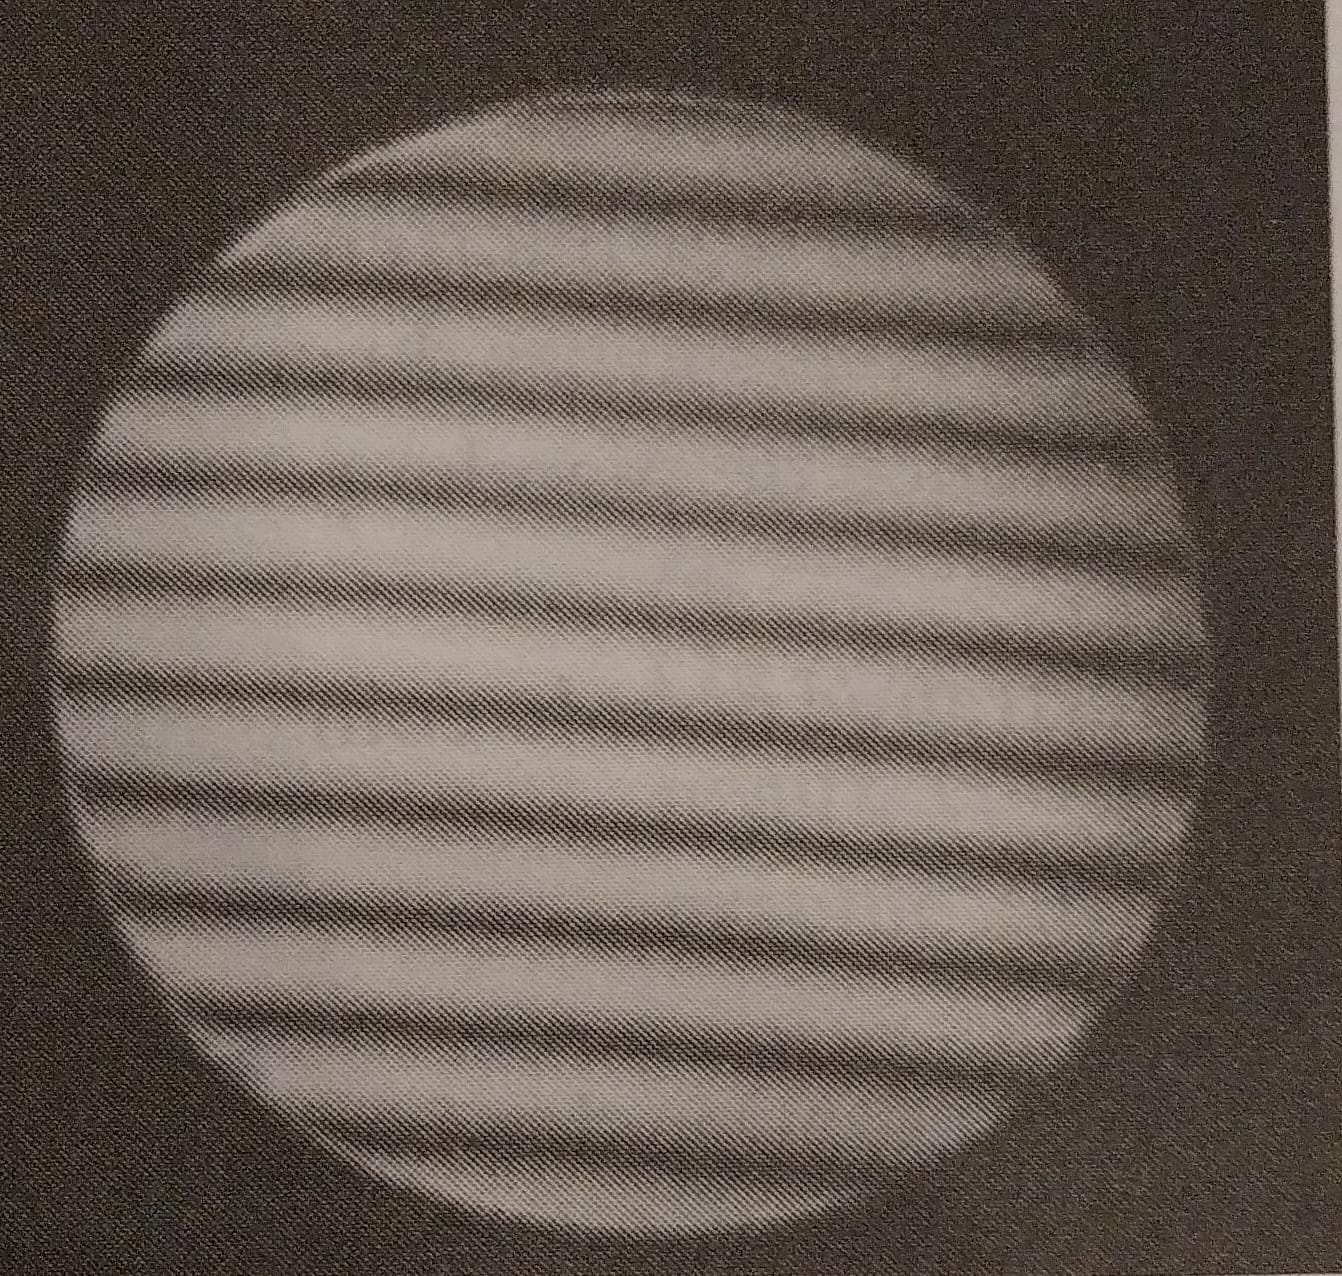
\includegraphics[width=\textwidth]{franges_egale_epaisseur.jpg}
      \caption{Franges d'égale épaisseur}                                              
  \end{subfigure}
  \begin{subfigure}[b]{0.3\textwidth}
      \centering
      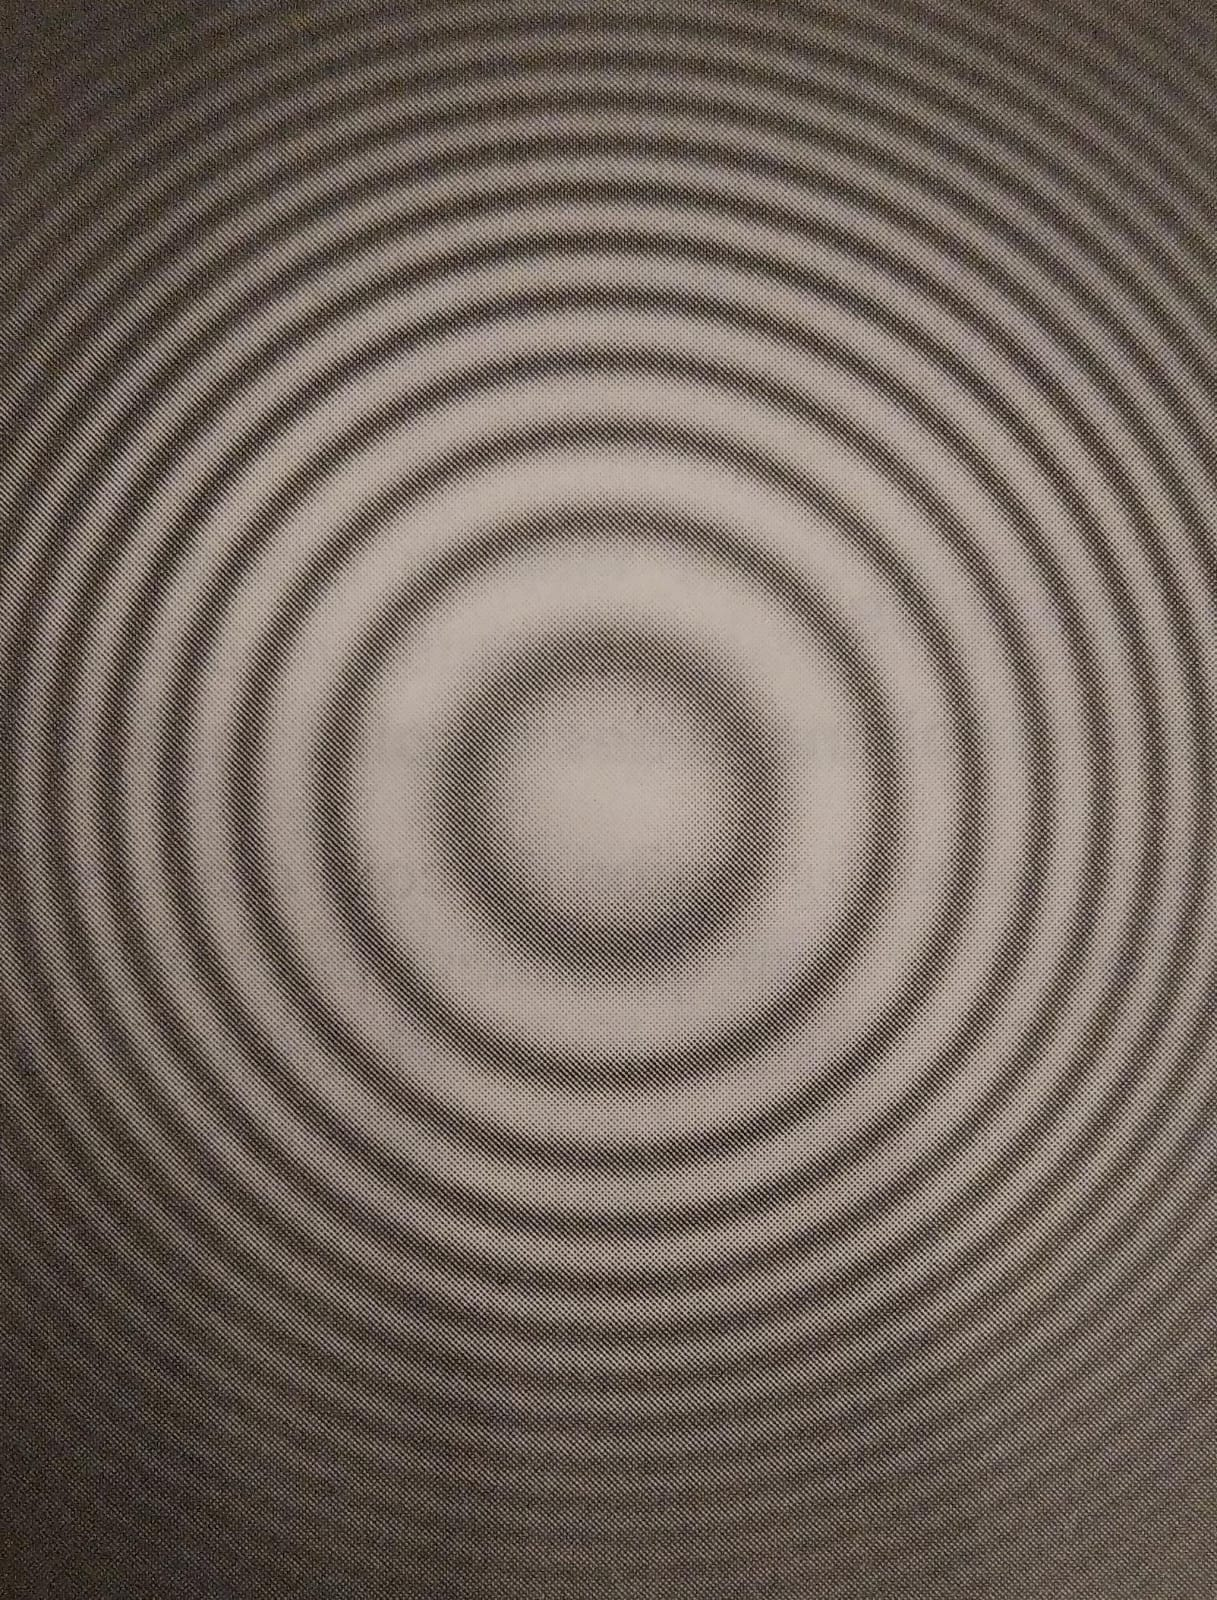
\includegraphics[width=\textwidth]{franges_anneaux.jpg}
      \caption{Franges d'égale inclinaison }
      \label{fig:franges_egales_epaisseur}
  \end{subfigure}}
  \caption{Les observations associées aux différents réglages}
\end{figure}


\newpage


\textbf{Anecdote: } L'interféromètre de Michelson a à la base été construit pour tenter de détecter la présence de l'éther, un gaz hypothétique qui devait servir de support à la propagation des ondes électromagnétiques.
L'idée était de mesurer la vitesse de la lumière dans deux directions perpendiculaires et de tenter de détecter des variations, qui auraient été dues à la présence de l'éther.
L'expérience fut un échec, dans le sens où elle ne permit pas de détecter l'éther, et Michelson conclut que le vent de l'éther était soit petit, soit inexistant.

\section{Anneaux d'égale inclinaison}

Un interféromètre de Michelson est réglé en lame d'air et éclairé avec une lampe à vapeur de sodium, qu'on considérera monochromatique, de longueur d'onde $\lambda = 589nm$.
On observe sur un écran un ensemble d'anneaux concentriques (voir Fig \ref{fig:franges_egales_epaisseur}). 
\begin{enumerate}
  \item Préciser l'ensemble des réglages nécessaires à l'obtention des anneaux visibles sur la figure \ref{fig:franges_egales_epaisseur}. 
  \item Un logiciel permet de tracer le profil des niveaux de gris de la figure \ref{fig:franges_egales_epaisseur} selon un diamètre vertical. Le résultat est donné Fig. \ref{fig:niveaux_de_gris}.Trouver une relation entre le rayon d'un anneau et l'ordre d'interférence. En déduire la valeur $e$ de l'épaisseur entre les deux miroirs, sachant que les anneaux sont observé dans le plan focal d'une lentille convergente de distance focale $f'=1,00m$ placée en sortie de l'interféromètre.
  \item Si on réduit $e$ de moitié, combien d'anneaux vont défiler au centre de la figure d'interférences ?  
\end{enumerate}

\begin{figure}[h]
  \centering
  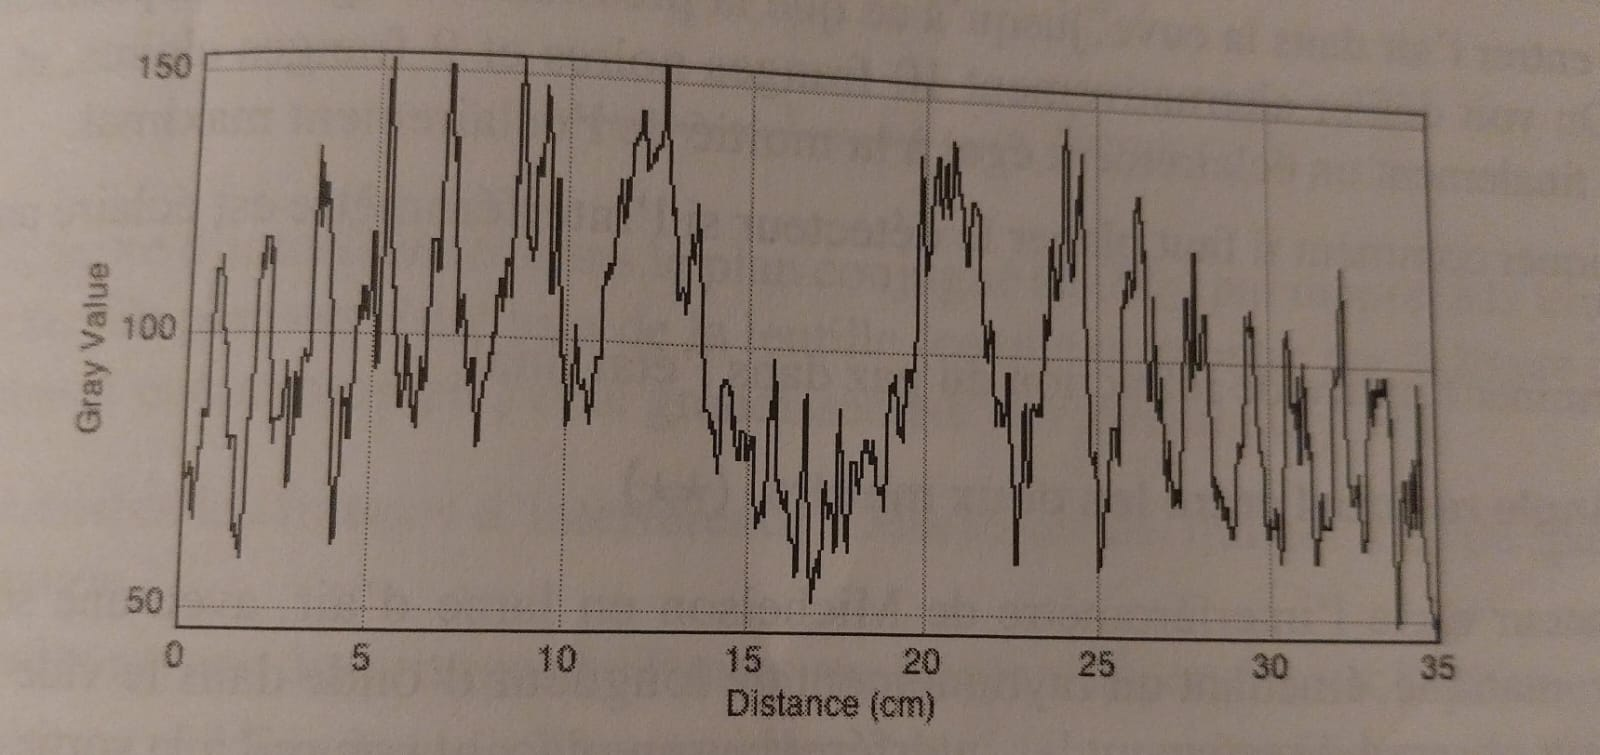
\includegraphics[width=0.5\textwidth]{niveaux_de_gris.jpg}
  \caption{Profil d'éclairement (l'axe des abscisses est en cm)}   
  \label{fig:niveaux_de_gris}
\end{figure}

\section{Problèmes de réglage}
Un opérateur règle l'interféromètre de Michelson en lame d'air, avec une source étendue monochromatique émettant un rayonnement de longueur d'onde $\lambda_0 = 589 nm$. 
L'opérateur observe les interférences à l'oeil, en "regardant au loin", car les franges sont situées à l'infini.
Il observe des anneaux d'égale inclinaison. 
Mais, quand l'observateur décale légèrement sa tête vers la droite ou la gauche, il voit les anneaux renter dans le centre. 
\begin{enumerate}
  \item Expliquer l'origine du problème et donner la solution pour le régler. 
  \item Majorer la valeur de l'angle résiduel sachant que l'observateur ne voit plus les anneaux défiler, et que les miroirs ont un diamètre de 40 mm. 
\end{enumerate}


\section{Mesure de l'écart du doublet jaune du sodium}


Un opérateur souhaite observer sur un détecteur des franges d'égale inclinaison grâce à un Michelson. 
Le Michelson est éclairé à l'aide d'une lampe à valeur de sodium. 
\begin{enumerate}
  \item Décrire le protocole expérimental pour obtenir des anneaux d'égale inclinaison sur le détecteur. 
  \item A partir du contact optique, on déplace le miroir mobile de l'interféromètre. Le détecteur enregistre des brouillages successifs ayant lieu tous les $d=0,29$mm. Justifier l'existence de ces brouillages successifs et en déduire l'écart de longueur d'onde du doublet du sodium, sachant que la longueur d'onde moyenne est $\lambda_m = 589,3$ nm. \\[1.5cm]
\end{enumerate}

\begin{figure}[h]
  \centering
  
\includegraphics[width=0.27\textwidth]{michelson .jpg}

  
\end{figure}
\end{document}

